% ********************************************************
%   ROSARIO
%   Texto y musica con acompa\~namiento
%   by serachsam
% ********************************************************

% - Preambulo
\documentclass[12pt, letterpaper]{report}

%%% - Paquetes
\usepackage[spanish]{babel}
\usepackage[utf8]{inputenc}
\usepackage[T1]{fontenc}
\usepackage{xcolor}
\usepackage{pifont}
\usepackage{lettrine}
\usepackage{lmodern}
\usepackage{enumitem}
% Utilizamos el paquete para gestionar imagenes jpg
\usepackage{graphicx}
\graphicspath{ {images/} }

\oddsidemargin -1.0cm
\headsep -1.0cm
\textwidth=18.5cm
\textheight=23cm

\setlength{\parskip}{\baselineskip}

\setcounter{secnumdepth}{0}
\setcounter{tocdepth}{4}


%% Portada del Libro

%% Portada del Libro
\title{
  \textbf{ \Huge CORONILLA } \\
  \LARGE Rosario de la Virgen María %\\
  %\vspace{2em}
  %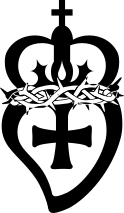
\includegraphics{logo}
}

%\author{ \Large{ \textbf{Linda Isabel Mart\'inez Castro \\ Samuel Jos\'e Guti\'errez Avil\'es} } }

\author{ 
  \Large \textbf{Linda Isabel Mart\'inez Castro} \\ 
  \Large \textbf{Samuel Jos\'e Guti\'errez Avil\'es}
}

\date{ \LARGE \small \textit{2019 - 2021} }

\begin{document}
    %%\pagenumbering{gobble}
    %%\pagestyle{plain}

    %% - Portada
    \maketitle
    
    %% - Indice
    \LARGE ÍNDICE GENERAL

    \large \hfill{Página}\\
    \Large \textbf{Introducción \hfill{2}}\\
    .\hspace{1cm} \large Historia \dotfill 3\\
    .\hspace{1cm} \large Acerca del Rorasio y su Rezo \dotfill 3\\
    .\hspace{2cm} \large \textit{Historia del Rosario} \dotfill 3\\
    .\hspace{2cm} \large \textit{Indulgencias} \dotfill 6\\
    .\hspace{1cm} \large Como rezar el Rosario \dotfill 7\\
    .\hspace{2cm} \large \textit{Ofrecimiento} \dotfill 7\\
    .\hspace{2cm} \large \textit{Persignarse} \dotfill 7\\
    .\hspace{2cm} \large \textit{Credo} \dotfill 8

    \noindent
    \Large \textbf{Ordinario de la Misa \hfill{9}}\\
    .\hspace{1cm} \large Señor ten piedad \dotfill 10\\
    .\hspace{1cm} \large Gloria a Dios en lo alto del cielo \dotfill 16\\
    .\hspace{1cm} \large Creo en Dios \dotfill 26\\
    .\hspace{1cm} \large Santo \dotfill 39\\
    .\hspace{1cm} \large Cordero de Dios \dotfill 48

    \noindent
    \Large \textbf{Propio de la Misa \hfill{57}}\\
    .\hspace{1cm} \large Canto de Entrada \dotfill 58\\
    .\hspace{1cm} \large Melodia Responsorial \dotfill 69\\
    .\hspace{2cm} \large \textit{Ciclo A} \dotfill 69\\
    .\hspace{2cm} \large \textit{Ciclo B} \dotfill 79\\
    .\hspace{2cm} \large \textit{Ciclo C} \dotfill 86\\
    .\hspace{1cm} \large Aclamaci\'on al Evangelio \dotfill 93\\
    .\hspace{1cm} \large Presentación de Ofrendas \dotfill 98\\
    .\hspace{1cm} \large Canto de Comunion \dotfill 112\\
    .\hspace{1cm} \large Canto Final \dotfill 122
    \clearpage

    %% - Introduccion
    \begin{center}
        \vspace*{9cm}
        \textbf{\Huge Introducci\'on}
    \end{center}
    \clearpage
    
    \LARGE HISTORIA
    
    \Large Esta musica nacio de las ganas no caer en la monotonia al rezar el Rosario. Un d\'ia simplemente pensamos: <<?`Porque no lo hacemos cantado?>> Recordamos diferente tonos en los que habias 
    escuchado que se cantaban las diferentes partes, pero no habia una melodia o tono coherente en todo el recorrido del rezo. 
    Sin más nos decidimos de hacer una melodia completa.
    
    Junto con escuchar las diferentes versiones gregorias e investigar que textos se musicalizarian nos decidimos por hacer un sola melodia homogenia para todo el <<Rosario>>, que fuera facil de interpretar y de recordar.
    
    \LARGE HACERCA DEL ROSARIO Y SU REZO
    
    \LARGE \textit{Historia del Rosario}
    
    \Large Existen diversas explicaciones sobre como surgio el rezo de <<El Rosario>>, todas validas y loables, como esta:
    
    \Large \textit{<<En la antigüedad, los romanos y los griegos solían coronar con rosas a las estatuas que representaban a sus dioses como símbolo del sufrimiento de sus corazones. Siguiendo esta tradición, las mujeres cristianas que eran llevadas al martirio por los romanos, marchaban por el coliseo vestidas con sus ropas más vistosas y con sus cabesas adornadas con coronas de rosas, como símbolo de alegría y de la entrega de sus corazones al ir al encuentro de Dios. Por la noche, los cristianos recogían sus coronas y por cada rosa, recitaban una oración o un salmo por el eterno descanso del alma de las mártires por eso se llama Rosaro. La palabra ``Rosario'' significa ``Corona de Rosas''. La Iglesia recomendó rezar el ``Rosario'', el cual consistía en recitar los 150 salmos de David, pues era considerada una oración sumamente agradable a Dios y fuente de innumerables gracias para aquellos que la rezaran. Sin embargo, esta recomendación sólo la seguían las personas cultas y letradas, pero no la mayoría de los cristianos. Por esto, la Iglesia sugirió que aquellos que no supieran leer, suplantaran los 150 salmos por 150 Avemarías, divididas en quince decenas. A este ``Rosario corto'' se le llamó ``El salterio de la Virgen''.>>} \cite{RorasioCatholicNet}
    
    \Large O esta otra:
    
    \Large \textit{<<El rezo del ``Santo Rosario'' surge aproximadamente en el año 800 a la sombra de los monasterios, como ``Salterio de los laicos''. Dado que los monjes rezaban los 150 salmos de David, a los laicos, los cuales en su mayoría no sabían leer, se les enseñó a rezar 150 Padres Nuestros. Al pasar el tiempo, se formaron otros tres salterios con 150 Aves Marías, 150 alabanzas en honor de Jesús y 150 alabanzas en honor de María. En el año 1365 se hizo una combinación de los cuatro salterios, dividiendo las 150 Aves Marías en 15 decenas y poniendo un Padre nuestro al inicio de cada una de ellas. En 1500 se estableció, para cada decena, la meditación de un hecho de la vida de Jesús o María, y así surgió el actual Rosario de quince misterios. La palabra Rosario significa ``Corona de Rosas''. La Virgen María ha revelado a muchas personas que cada vez que rezan un Ave María le entregan una rosa y por cada Rosario completo le entregan una corona de rosas. La rosa es la reina de las flores, así que el Rosario es la rosa de todas las devociones y por lo tanto es la más importante.>>}\cite{AciPrensaRosario}
    
    \Large Dependiendo de la fuente que se consulte, pero es cierto que su devocion empezó así:
    
    \Large \textit{<<A finales del siglo XII, se le apareció la Virgen a Santo Domingo de Guzmán y le dijo que la mejor arma para convertir a las almas duras no era con el rezo de su salterio. Santo Domingo realizo varios milagros Toulouse mientras rezar el salterio de la Virgen convirtiendo muchas personas. Santo Domingo murió en 1221, después de una vida en la que se dedicó a predicar y hacer popular la devoción del <<Rosario>> entre las gentes de todas las clases sociales para el sufragio de las almas del Purgatorio, para el triunfo sobre el mal y prosperidad de la Santa Madre de la Iglesia. El rezo del Rosario mantuvo su fervor por cien años después de la muerte de Santo Domingo y empezó a ser olvidado. En 1349, hubo en Europa una terrible epidemia de peste a la que se le llamó ``La muerte negra'' en la que murieron muchísimas personas. Fue entonces cuando el fraile Alan de la Roche, superior de los dominicos en la misma provincia de Francia donde había comenzado la devoción al Rosario, tuvo una aparición, en la cual Jesús, la Virgen y Santo Domingo le pidieron que reviviera la antigua costumbre del rezo del Santo Rosario. El Padre Alan comenzó esta labor de propagación junto con todos los frailes dominicos en 1460. Ellos le dieron la forma que tiene actualmente, con la aprobación eclesiástica. A partir de entonces, esta devoción se extendió en toda la Iglesia.>>}\cite{RorasioCatholicNet}
    
    \Large Y que en la actualidad la iglesia ve <<El Rosario>> de esta manera:
    
    \Large ``El Rosario de la Virgen María, difundido gradualmente en el segundo Milenio bajo el soplo del Espíritu de Dios, es una oración apreciada por numerosos Santos y fomentada por el Magisterio. En su sencillez y profundidad, sigue siendo también en este tercer Milenio apenas iniciado una oración de gran significado, destinada a producir frutos de santidad. Se encuadra bien en el camino espiritual de un cristianismo que, después de dos mil años, no ha perdido nada de la novedad de los orígenes, y se siente empujado por el Espíritu de Dios a «remar mar adentro» (duc in altum!), para anunciar, más aún, 'proclamar' a Cristo al mundo como Señor y Salvador, «el Camino, la Verdad y la Vida» (Jn14, 6), el «fin de la historia humana, el punto en el que convergen los deseos de la historia y de la civilización». El Rosario, en efecto, aunque se distingue por su carácter mariano, es una oración centrada en la cristología. En la sobriedad de sus partes, concentra en sí la profundidad de todo el mensaje evangélico, del cual es como un compendio. En él resuena la oración de María, su perenne Magnificat por la obra de la Encarnación redentora en su seno virginal. Con él, el pueblo cristiano aprende de María a contemplar la belleza del rostro de Cristo y a experimentar la profundidad de su amor. Mediante el Rosario, el creyente obtiene abundantes gracias, como recibiéndolas de las mismas manos de la Madre del Redentor.''\cite{Enciclica}
    
    \LARGE \textit{Indulgencias}
    
    \Large ``Para fomentar esta proyección eclesial del Rosario, la Iglesia ha querido enriquecerlo con santas indulgencias para quien lo recita con las debidas disposiciones.''\cite{Enciclica}
    
    Es tan grande el aprecio que la Iglesia ha tenido por el Rezo del Rosario que los Papas han concedido muchas indulgencias a lo largo de la historia. Acontinuación Detallaremos alguas:

    \begin{enumerate}
      \item Se concede indulgencia plenaria al fiel cristiano que:
      \begin{itemize}
        \item Rece devotamente el Rosario mariano en una iglesia u oratorio, o en familia, en una comunidad religiosa, en una asociación piadosa y, en general, en cualquier reunión de fieles.\cite{Indulgencias}
        \item Se una devotamente al rezo de esta plegaria llevado a cabo por el Sumo Pontífice y retransmitida por radio o por televisión.\cite{Indulgencias}
      \end{itemize}
      \item El fiel cristiano puede ganar una indulgencia si usa con devoción algún objeto de piedad (crucifijo o cruz, rosario, escapulario, medalla) debidamente bendecido.
      \item Son dignas de especial mención las concesiones que se refieren a algunas obras, enriquecidas con indulgencia plenaria, con las cuales el fiel cristiano puede ganarla todos los días del año:
      \begin{itemize}
        \item La adoración del Santísimo Sacramento durante al menos media hora.\cite{Indulgencias}
        \item El piadoso ejercicio del Via Crucis.\cite{Indulgencias}
        \item El rezo del Rosario mariano o del himno Akhátistos en una iglesia o un oratorio, o en familia, en una comunidad religiosa, en una asociación piadosa y, en general, siempre que varios fieles se reúnan para un buen fin.\cite{Indulgencias}
        \item La lectura piadosa de la Sagrada Escritura durante al menos media hora.\cite{Indulgencias}
      \end{itemize}
    \end{enumerate}
    
    \LARGE COMO REZAR EL ROSARIO

    \Large Las diferentes partes propuestas a continuaci\'on siguen la estructura propuesta por el Papa San Juan Pablo II en su Carta Apostólica <<Rosarium Virginis Mariae>>:
    
    \LARGE \textit{1. Ofrecimiento.}
    
    \Large Intención por la cual se reza el rosario, puede ser por un difunto, las animas del Purgatorio o una situación en particular; para pedir una gracia, una virtud a imitar o un pecado a evitar. Puede hacerse en silencio si se reza solo.
    
    \textit{<<Ofresco(Ofrecemos) el rezo de este rosario por: ...>>}
    
    \LARGE \textit{2. Persignarse}
    
    \Large Hacer la señal de la cruz sobre la frente, la cara y el pecho. 
    
    \textit{<<Por la señal de la Santa Cruz de nuestro enemigos libranos Señor, Dios nuestro. En el nombre del Padre y del Hijo y del Esperítu Santo.>>}
    
    \LARGE \textit{3. Credo}
    
    \Large Sujetando el <<Rosario>> por el crucifijo se reza el Credo Apostólico.
    
    \textit{<<Creo en Dios Padre, todopoderoso, creador del cielo y de la tierra.\\
    Creo en Jesucristo, su único Hijo, nuestro Señor, que fue concebido por obra y gracia del Espíritu Santo, nació de Santa María Virgen, padeció bajo el poder de Poncio Pilato, fue crucificado, muerto y sepultado, descendió a los infiernos, al tercer día resucitó entre los muertos, subió a los cielos y está sentado a la derecha de Dios Padre, todopoderoso. Desde allí vendrá a juzgar a vivos y a muertos.\\
    Creo en el Espíritu Santo, la Santa Iglesia Católica, la comunión de los santos, el perdón de los pecados, la resurrección de la carne y la vida perdurable. Amén.>>}
    
    \LARGE \textit{3. Acto de Contrición}
    
    \Large Existen diversas oraciones del penitente, las más común el <<Yo Confieso>>, cualquiera es valida, pero usaremos la siguiente:
    
    \textit{<<¡Señor mío, Jesucristo! Dios y Hombre verdadero, Creador, Padre y Redentor mío; por ser Vos quien sois, Bondad infinita, y porque os amo sobre todas las cosas, me pesa de todo corazón haberos ofendido; también me pesa porque podéis castigarme con las penas del infierno. Ayudado de vuestra divina gracia propongo firmemente nunca más pecar, confesarme y cumplir la penitencia que me fuere impuesta. Amén.>>}
    
    \begin{enumerate}
        \item Padre Nuestro
        \item Ave Mar\'ia
        \item Letanias Lauretanas
        \item Salve
        \item Oraci\'on Final
    \end{enumerate}
    \clearpage
    
    %\begin{lilypond}%[staffsize=20]
    %    \include "../partes/persignarse.ly"
    %\end{lilypond}
    %\clearpage
    
    %\begin{lilypond}%[staffsize=20]
    %    \include "../partes/credo.ly"
    %\end{lilypond}
    %\clearpage
    
    %\begin{lilypond}%[staffsize=20]
    %    \include "../partes/acto_contriccion.ly"
    %\end{lilypond}
    %\clearpage
    
    %\begin{lilypond}%[staffsize=20]
    %    \include "../partes/padre_nuestro.ly"
    %\end{lilypond}
    %\clearpage
    
    %\begin{lilypond}%[staffsize=20]
    %    \include "../partes/ave_maria.ly"
    %\end{lilypond}
    %\clearpage
    
    %\begin{lilypond}%[staffsize=20]
    %    \include "../partes/letanias.ly"
    %\end{lilypond}
    %\clearpage
    
    %\begin{lilypond}%[staffsize=20]
    %    \include "../partes/salve.ly"
    %\end{lilypond}
    %\clearpage
    
    %\begin{lilypond}%[staffsize=20]
    %    \include "../partes/oracion_final.ly"
    %\end{lilypond}
    %\clearpage
    
    \begin{thebibliography}{0}
      \bibitem{RorasioCatholicNet} http://www.rosario.catholic.net/index.php
      \bibitem{AciPrensaRosario} https://www.aciprensa.com/Rosario/surgio.htm
      \bibitem{Enciclica} Carte Apostólica Rosarium Virginis Mariae del sumo pontífice San Jaun Pablo II
      \bibitem{Indulgencias} Manual de Indulgencias Enchiridion indulgentiarum
    \end{thebibliography}
\end{document}
 
